\documentclass[manuscript, screen, review, acmsmall, anonymous]{acmart}
%\documentclass[acmsmall,authorversion]{acmart}
\usepackage{subcaption}
\usepackage{hyperref}
\usepackage{booktabs}
\usepackage{pifont}
\usepackage[dvipsnames,table]{xcolor}
\usepackage{colortbl}        % For color in tables
\usepackage{adjustbox}

\usepackage{pdflscape}

\newcommand{\TODO}[1]{\textcolor{red}{#1}}

\usepackage[skins, breakable]{tcolorbox}
%% \BibTeX command to typeset BibTeX logo in the docs
\AtBeginDocument{%
  \providecommand\BibTeX{{%
    Bib\TeX}}}

\begin{document}

\title{Generative AI and Creativity: A Systematic Literature Review and Meta Analysis}

\author{Niklas Holzner}
\email{n.holzner@campus.lmu.de}
\affiliation{
  \institution{LMU Munich}
  \city{Munich}
  \state{Bavaria}
  \country{Germany}
}
\author{Sebastian Maier}
\email{maier.sebastian@campus.lmu.de}
\affiliation{
  \institution{LMU Munich \& Munich Center for Machine Learning (MCML)}
  \city{Munich}
  \state{Bavaria}
  \country{Germany}
}
\author{Stefan Feuerriegel}
\email{feuerriegel@lmu.de}
\affiliation{
  \institution{LMU Munich \& Munich Center for Machine Learning (MCML)}
  \city{Munich}
  \state{Bavaria}
  \country{Germany}
}
\begin{abstract}
Generative artificial intelligence (GenAI) is increasingly used to support a wide range of human tasks, yet empirical evidence on its effect on creativity remains scattered. Can GenAI generate ideas that are creative? To what extent can it support humans in generating ideas that are both creative and diverse? In this study, we conduct a meta-analysis to evaluate the effect of GenAI on the performance in creative tasks. For this, we first perform a systematic literature search, based on which we identify $N$ = XX relevant studies for inclusion in our meta-analysis. We then compute standardized effect sizes based on Hedges' $g$. We compare different outcomes: (i)~how creative GenAI is; (ii)~how creative humans augmented by GenAI are; and (iii)~the diversity of ideas by humans augmented by GenAI. Our results indicate a small, statistically non-significant improvement in human creative performance ($g$ = X.XX), and a comparable but statistically significant creative performance for humans supported by GenAI ($g$ = X.XX). Further, GenAI has a positive effect on the diversity of ideas for such collaborations between humans and GenAI ($g$ = X.XX). We further analyze heterogeneity across different types of GenAI models (e.g., text-to-text, text-to-image), different tasks (e.g., creative writing, ideation), different measurements (e.g., novelty, originality), and different participant populations (e.g., laypeople vs. domain experts). Overall, our results position GenAI as an augmentative tool that can support, rather than replace, human creativity---particularly in tasks benefiting from ideation support.
\end{abstract}

\maketitle
\section{Introduction}
\label{sec:Introduction}

% Gen AI

Generative artificial intelligence (GenAI) refers to a class of machine learning technologies that have the capability to generate new content that resembles human-created output, such as images, text, audio, and videos  \cite{FeuerriegelBISE2024}. GenAI can thus support various human tasks such as writing, software development, composing lyrics, and academic research, often at a performance similar to that of humans \TODO{add: https://journals.aom.org/doi/10.5465/amj.2023.4006}\cite{Herbold2023, Cui2025, 10.1093/pnasnexus/pgae052, Ruksakulpiwat2024, brynjolfsson2024generativeaiwork}. On top of that, Generative AI has also become a valuable tool in creative industries---spanning graphic design, advertising, fashion, writing, and visual arts  \TODO{Eine Ref von Jochen Hartmann/TUM
plsu: https://pubsonline.informs.org/doi/10.1287/mksc.2023.0494}\cite{Sun_2024}. 

Yet, empirical evidence on the benefits of GenAI for creative performance is scattered, and the theoretical arguments are often inconsistent or even contradictory. On the one side, cognitive research argues that creativity is an inherently human trait \cite{aru2024artificialintelligenceinternalprocesses,sæbø2024stochasticshumanartificialcreativity}. One common issue in practice is that GenAI models often lack the tacit knowledge required for systematic, compositional reasoning such as multi-step problem solving to generate ideas perceived as creative, especially in real-world tasks from businesses. Similarly, GenAI is likely to reproduce ideas seen during training rather than ideating novel ideas \cite{ismayilzada2024creativityaiprogresseschallenges}. Hence, simply by means of the training data of GenAI, the generated ideas may also be less diverse than those of humans \cite{doi:10.1126/sciadv.adn5290}. On the other side, there is early evidence suggesting that outputs from GenAI are perceived as being creative \cite{wang2024aicreativehumans}. For example, several studies find benefits from GenAI in creative tasks, but these findings are typically limited to specific creative tasks (e.g., story writing, ideating business models) \cite{doi:10.1126/sciadv.adn5290, Lee2024, Zhou2024, Wadinambiarachchi_2024}. This may suggest that GenAI can generally improve creativity but it is often unclear how well the results generalize across domains.  

Here, we perform a meta-analysis to evaluate the effect of GenAI on creative performance.\footnote{Code and data for review are available via \TODO{Anonymized Git}. Upon acceptance, we will move both code and data to a public GitHub repository.} For this, we focus on different outcomes, namely: (i)~how creative GenAI is; (ii)~how creative humans augmented by GenAI are; and (iii)~the diversity of ideas by humans augmented by AI.\footnote{We also considered a fourth outcome, namely, the diversity of ideas generated by humans with GenAI support. Yet, our literature search did not return a sufficient number of empirical studies for this outcome. Hence, we refrain from analyzing this outcome. However, we identify this gap as a promising opportunity for future research, which we elaborate on in the discussion section.} To this end, we analyze the following \textbf{research questions (RQs)}:

\begin{itemize}
\item \textbf{RQ1:} \textit{How creative are ideas generated by GenAI (compared to humans without GenAI support)?}
\item \textbf{RQ2a:} \textit{How creative are ideas generated by humans when supported by GenAI (compared to humans without GenAI support)?}
\item \textbf{RQ2b:} \textit{How diverse are ideas generated by humans when supported by GenAI (compared to humans without GenAI support)?}
\end{itemize}

\noindent
To answer the above research questions, we first perform a systematic literature search and then conduct a meta-analysis. Overall, we retrieved $N= 693$ studies for inclusion, and eventually identified $N = TBA$ studies with empirical results. We then calculated the standardized effect size Hedges' $g$ and computed a random-effects meta-analysis. \TODO{hetoergeneity IMHO raus nehmen, nur potential bias (aber vlt kan under sastz auch ganz weg bzw. in wine klammer => ich ahbe ja am Ende den querverweis für anhang }We conduct several sensitivity analyses, meta-regressions, and Egger's tests to address heterogeneity and potential bias. We further ran a moderator analysis on study heterogeneity across different GenAI model types (e.g., text-to-text, text-to-image), different tasks (e.g., creative writing, ideation), and different participant populations (e.g., laypeople vs. domain experts). to provide a general but differentiated understanding of the effect of GenAI on creativity. Additional robustness checks are reported in the \TODO{cross ref supplements}.

\begin{figure}
  \centering
  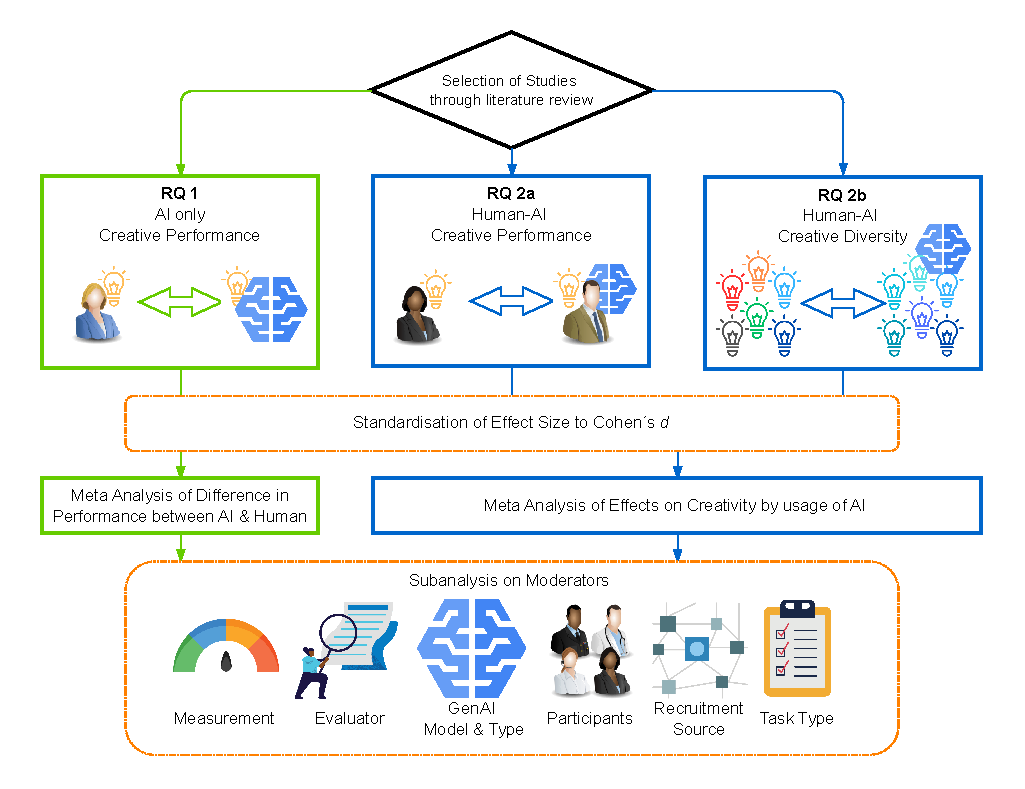
\includegraphics[width=0.9\linewidth]{overview.pdf}
  \caption{\textbf{Overview of the meta-analysis procedure.} We address three research questions: (RQ1) creative performance of GenAI alone, (RQ2a) creative performance of humans supported by GenAI, and (RQ2b) diversity of ideas in human-GenAI collaboration. After selecting studies via systematic literature review, we standardize effect sizes (Cohen's $d$) and conduct meta-analyses, including a moderator analysis to study heterogeneity across types of GenAI models, tasks, measurements, and participant populations.}
\end{figure}


\section{Methods}
\label{sec:Methods}

In this section, we describe our data collection to identify relevant studies and statistical analysis. 

\subsection{Search Strategy}

%Key definitions forming the basis for our understanding of creativity in the context of our meta analysis are \TODO{search included studies for creativity definitions}: 


% \begin{figure}[h!]
%     \label{fig:earch-query}
%   \centering
%   \begin{tcolorbox}[
%     enhanced,
%     breakable,
%     center upper, 
%     colback=gray!10,
%     colframe=gray!60!black,
%     boxrule=0.8pt,
%     arc=4pt,
%     outer arc=4pt,
%     drop shadow={black!50!white,opacity=0.3},
%     width=\textwidth,
%     title=\textbf{Creativity}
%   ]
%     \begin{verbatim}
%     novelty, originality, creativity
%     \end{verbatim}
%   \end{tcolorbox}
%   \caption{Definition of creativity for our meta-analysis.}
%   \label{fig:search-query}
% \end{figure}
% \begin{figure}[h!]
%     \label{fig:earch-query}
%   \centering
%   \begin{tcolorbox}[
%     enhanced,
%     breakable,
%     center upper, 
%     colback=gray!10,
%     colframe=gray!60!black,
%     boxrule=0.8pt,
%     arc=4pt,
%     outer arc=4pt,
%     drop shadow={black!50!white,opacity=0.3},
%     width=\textwidth,
%     title=\textbf{Creative diversity}
%   ]
%     \begin{verbatim}
%     cosine similarity
%     \end{verbatim}
%   \end{tcolorbox}
%   \caption{Definition of creative diversity for our meta-analysis.}
%   \label{fig:search-query}
% \end{figure}
    
\textbf{Search databases:} To ensure transparency, reproducibility, and quality of our meta-analysis, we follow the PRISMA 2020 framework for systematic literature reviews \TODO{PRISMA 2020 Checklist} \TODO{citation PRISMA Checklist}. To identify relevant studies, we searched the following databases: (i)~Web of Science, (ii)~SSRN, and (iii)~arXiv. Our search includes non-peer-reviewed studies to reflect the rapidly evolving nature of GenAI research and to capture recent advances. Our search was limited to publications in the English language from the past five years, which is loosely aligned with the emergence of foundational models such as GPT and BERT. The knowledge cutoff of our search is May 2, 2025.

\textbf{Search query:} Our search query is intentionally broad to include various ways to relate to GenAI technology and creativity. Overall, our search query is inspired by Schemmer et al.\,(2022) \cite{Schemmer2022} \TODO{citation Schemmer}, but which we adapted to our research question, namely, creativity:

  \begin{tcolorbox}[
    enhanced,
    breakable,
    center upper, 
    colback=gray!10,
    colframe=gray!60!black,
    boxrule=0.8pt,
    arc=4pt,
    outer arc=4pt,
    drop shadow={black!50!white,opacity=0.3},
    width=\textwidth,
    fontupper=\footnotesize,
    title=\textbf{Search query}
  ]
    \begin{verbatim}
    TITLE("creativity" OR "creative" OR "ideation" OR "idea")
    AND
    ("AI" OR "Artificial Intelligence" OR "LLM" OR "Large Language Models")
    \end{verbatim}
  \end{tcolorbox}

\textbf{Inclusion/exclusion:} The process for inclusion/exclusion in our systematic literature review is shown in Figure~\ref{fig:PRIMSAFlowchart} (based on the format of the PRISMA 2020 Flowchart \TODO{citation PRISMA Flowchart}). Literature screening, eligibility checks, and final inclusion were performed by one person (the first author). In the identification phase, $N$ = 691 publications were identified by our search query, out of which $n$ = 96 duplicate publications were removed manually. Out of the remaining $n$ = 595 publications, both the title and abstract were screened for inclusion in the assessment of eligibility. Here, \TODO{würde ich nicht unterscheiden (und auch im PRISMA bündeln) $n$ = 182 AND $n$ = 334} publications were excluded due to a lack of fit (e.g., a focus on legal studies). 

Subsequently,  $n$ = 79 records were assessed for eligibility. Studies were eligible if they:
\begin{enumerate}
  \item The study design was aimed at comparing (a)~the creativity performance of humans versus GenAI or (b)~the creative performance of humans with vs. without GenAI support. The study further followed a between-subject experiment design, which is crucial to make rigorous statistical comparisons. %As a result, we excluded studies with a different methodological focus (e.g., developing new software such as GenAI to prevent bias).  
  \item The study had to report sufficient statistics (e.g., the group means and standard deviations or equivalent statistics) that allow for computation of standardized effect size Hedges' $g$. In cases where such statistics were not directly reported, we examined whether the publication was accompanied by raw data, either in supplementary materials or associated repositories, that would enable us to reconstruct the necessary statistics. However, if these data were not accompanied by clearly documented analysis scripts and/or the reconstruction would have required substantial interpretation or rewriting of the original code, the study was excluded based on insufficient raw data.
  \item The study had to measure creative performance using an established measurement dimension (e.g., novelty \TODO{REF}, originality \TODO{REF}, diversity \TODO{REF}). 
%  \item Do not have the main topic of developing certain software or GenAI to prevent bias
  \item Do not provide raw data to prevent mistakes when handling unknown data
%  \item Are published in English
%  \item Are published within the last 5 years
%  \item Are peer-reviewed
%  \item Are openly accessible through our databases
\end{enumerate}
In this stage, publications were excluded due to (i)~insufficient study design ($n$ = 33) (ii)~insufficient statistics ($n$ = 8), (iii)~insufficient creativity measurement ($n$ = 4), and (iv)~\TODO{rename in prsima}insufficient raw data ($n$ = 2). Cases with ambiguity were resolved through discussion until consensus was reached (based on Author \#1 together with Author \#2 and Author \#3).


We contacted the corresponding authors from 15 publications via e-mail to address two of the above reasons for exclusion, namely, (ii) insufficient statistics and (iv) insufficient data reporting. If no response was received after the initial contact, a follow-up e-mail was sent to maximize the inclusion of eligible studies. As a result, we obtained sufficient additional information for inclusion from four studies ($n = 4$). All studies that did not elicit a response were excluded

Given the novel scope of the research question and the evolving terminology in the field, we recognized the possibility that the search strategy might overlook relevant studies. To address this, the authors manually included two additional studies that met all eligibility criteria but were not captured by the original database query.

In total, we identified $n = 29$ publications that met the eligibility criteria for inclusion in our meta-analysis. Several of these publications reported multiple experiments or included multiple outcome measures related to creativity and diversity. As a result, the 29 studies correspond to a total of 131 effect size estimates. \TODO{das oben im Prisma noch weg: Reports of included studies}



\begin{figure}[h]
  \centering
  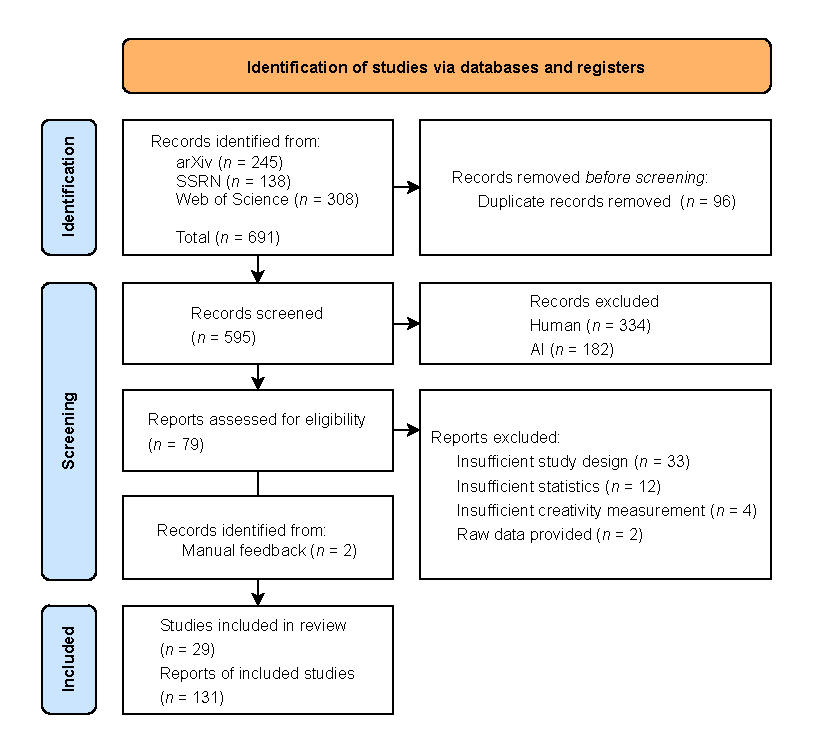
\includegraphics[width=.8\linewidth]{PRISMA_Flowchart}
  \vspace{-0.8cm}
  \caption{\textbf{PRISMA flow chart.}}
  \Description{PRISMA Flow Chart of the Literature Research.}
  \label{fig:PRIMSAFlowchart}
\end{figure}


\subsection{Data Collection}


The $n$ = 29 studies that met the inclusion criteria were recorded in our database. To ensure transparency and reproducibility, our database capturing all relevant study features and outcomes is deposited in our project repository. 

An overview of the extracted dimensions is summarized in Table~\ref{tab:variables}, which serves as the basis for exploring heterogeneity in creative performance across various study and task characteristics. Specifically, we extracted study-level data of metadata (title, author, abstract, publication date, source). We further provide details about the experimental design  (task type, GenAI type, GenAI model, creativity measurement, measurement evaluator), participant characteristics (recruitment source, professional domain), and outcome statistics (means, $SD$, $SE$, $n_\mathrm{total}$, $n_\mathrm{control}$, $n_\mathrm{treatment}$, $F$-value, standardized $\beta$, and $SE-\beta$). We discuss a few relevant dimensions in the following.

The \textbf{task type} reflects the notion that different creative tasks tap into distinct aspects of creativity (and thus different cognitive processes), such as compositional skills, imaginative reasoning, or divergent thinking (i.e., the ability to generate multiple, varied ideas in response to an open-ended prompt). The studies in our analysis employ a variety of creative tasks, each targeting different dimensions of creative cognition. For example, the so-called \emph{alternate uses task} (AUT) \TODO{REF} asks participants to generate unconventional uses for everyday objects (e.g., ``a brick''), which assesses originality. The so-called \emph{consequences task (CT)} \TODO{REF} involves imagining outcomes of improbable scenarios (e.g., ``What would happen if people could fly?''), which taps into imaginative thinking and hypothetical reasoning. The so-called \emph{divergent association task (DAT)} \TODO{REF}  requires listing unrelated words (e.g., ``apple'', ``justice'', ``galaxy''). \textit{Forward flow} (FF) measures \TODO{REF}  the conceptual distance between sequential thoughts in open-ended responses, reflecting the natural flow of creative ideation. Finally, other studies rely upon creative writing tasks such as short story composition or poetry to challenge narrative creativity, but also business ideation tasks (e.g., coming up with a new business model).


Creative performance is inherently multidimensional \TODO{SEBASTIAN: falls du hier noch was der psychology zum ziteieren hast, greatly appreciated}, and \textbf{creativity measurements} can be obtained in subjective (e.g., human ratings) or objective (e.g., via metrics from natural language processing such as semantic distance or cosine similarity \TODO{cite:}https://www.nature.com/articles/s44159-024-00392-z) ways. Subjective assessments often involve different rating scales, such as perceived creativity, originality, or novelty---each reflecting distinct psychological constructs. \TODO{SEBASTIAN: falls du hier noch was der psychology zum ziteieren hast, greatly appreciated}For example, \emph{creativity} is often perceived as a combination of novelty and effectiveness, \emph{originality} refers to how uncommon or unique an idea is, and \emph{novelty} emphasizes newness or unfamiliarity. These dimensions may be interpreted differently by human raters, depending on context and individual experience, because of which we also coded the identity of the \textbf{evaluator}. For example, self-assessments may introduce bias due to over- or underestimation of one's performance, while expert ratings tend to be more consistent and informed. Rule-based or AI-based evaluations offer standardization and scalability but may miss nuanced judgment or (tacit) domain knowledge. 

%As such, measurements, especially when asking human evaluators for a judgment, can also tap into different scales (e.g., perceived creativity, perceived oginality, perceived novelty). etc. [ADD in paretnhis a definition of how thee may be different perceived by humans] Evaluator: Who evaluates creativity matters greatly. Self-assessments may be biased, expert ratings are often more reliable, and AI or rule-based systems offer standardized evaluat. Importantly, the studies also vary in the choice of the evaluator, with some asking experts for evaluation, others focus on self-assesment or rule-based or AI evaluations. 



In cases where studies reported multiple measurements per experiment, we prioritized evaluations of creative performance by experts (over self-assessments). When multiple experiments were reported within a single study, each experiment was included separately, with one outcome measurement per experiment. Creative performance was encoded using the most conceptually appropriate metric available---ideally an overall creativity score (if available) or, alternatively, measures of originality or novelty before using any other measurement.\footnote{To examine potential heterogeneity across different conceptualizations of creative performance, we conducted exploratory subgroup analyses based on the specific constructs used—namely, creativity, originality, and novelty. However, these analyses revealed no substantial heterogeneity. This may be due to the high conceptual overlap among the constructs of creativity, originality, and novelty, which are often used interchangeably in both academic and applied contexts. We thus omitted the analysis for space but the reproducibility code is available for interested readers in our repository.}

 

\begin{table}[H]
  \centering
  \caption{\textbf{Extracted dimensions.}\label{tab:variables}}
  \vspace{-0.4cm}
  \footnotesize
  \begin{tabular}{@{\extracolsep{\fill}} l  p{0.7\linewidth} }
    \toprule
    \textbf{Dimensions} & \textbf{Values} \\
    \midrule
    GenAI type & text-to-text (T2T), text-to-image (T2I) \\
    \midrule
    GenAI model & GPT-4o, GPT-4, GPT-4all, GPT-3.5-turbo, GPT-3.5, GPT-3, Claude, SparkDesk, Qwen, Dou\,Bao, alpaca, bing, dolly, koala, oa, stablelm, vicuna, not disclosed (n.d.); \textit{optional:} multiple models \\
    \midrule
    Participants & Academia, business, laypeople, not disclosed \\
    \midrule
    Recruitment source & University, Prolific, Mturk, Public, Company \\
    \midrule
    Task type & alternate uses task (AUT), consequences task (CT), divergent associations task (DAT), forward flow (FF), creative writing, creative problem solving, creative thinking, divergent thinking, ideation product, ideation item usage, ideation research proposal, ideation business concepts, ideation other\\
    \midrule
    Creativity measurement & creativity scale, originality scale, novelty scale, semantic distance, cosine similarity, creative problem-solving scale, flexibility score \\
     \midrule
    Evaluator & self-assessed, laypeople, expert, rule-based, AI \\
    \addlinespace
    \bottomrule
  \end{tabular}
\end{table}

\subsection{Statistical Analysis}
\label{sec:StatAnalysis}

For each comparison, we extracted reported Cohen's $d$ or calculated it based on reported statistics \TODO{Cohens d citation}. When effect sizes were not directly reported, we converted other statistical measures (e.g., $t$-values, $F$-values, means and standard deviations) to Cohen's $d$ using widely accepted conversion formulas \TODO{citation other conversion ways}, which are documented in our the project repository. To adjust for potential upward bias in small samples, we applied Hedges' $g$ correction \cite{Hedges1985}\TODO{citation Hedges}. We report one effect size per individual experiment across all included studies to ensure statistical independence.

As we expect large heterogeneity regarding treatment, task, and measurement across studies, we chose to estimate a random-effects model as recommended by Cochrane \TODO{citation Cochrane}. Pooled effect sizes were estimated under the random-effects model using the DerSimonian-Laird estimator \cite{DerSimonian1986}\TODO{citation DerSimonian} to account for the expected between-study heterogeneity. We calculated 95 \% prediction intervals to indicate the expected range of true effects across settings. 


The variability in effect sizes across studies was quantified using the $I^2$ statistic, Cochran's $Q$ test, and by estimating the between-study variance ($\tau^2$) via Jackson's method \TODO{citation Jackson}. 

\textbf{Heterogeneity analysis:} To further explore potential sources of heterogeneity, we conducted subgroup analyses, such as comparing creativity across participants with different backgrounds (e.g., academic vs. business), to examine differential performance in GenAI-assisted creative tasks. As a robustness check, we also performed meta-regression analyses \TODO{REF}, which yielded results consistent with the subgroup analyses. For reasons of space, detailed meta-regression results are omitted.

\textbf{Bias assessment:} Risk of bias was assessed using Cochrane Risk-of-Bias 2.0 \TODO{complete RoB 2} tool, with judgments recorded for selection, performance, detection, and reporting bias \TODO{citation Cochrane Risk-of-Bias 2.0}. Publication bias was evaluated through Egger's regression test \TODO{cite} and the trim-and-fill procedure \TODO{cite} for comparisons including at least ten studies \TODO{citation Egger's regression test and the trim-and-fill procedure}. These analyses revealed no substantial concerns regarding bias; we thus omitted full results for brevity.


%meta-regression and analysis of raw data distribution were examined to determine whether effect sizes varied by task type (e.g., divergent thinking vs.\ writing tasks), creativity measurement (e.g., originality vs.\ novelty), measurement evaluator (e.g., automated vs.\ expert), GenAI models (GPT-4o vs.\ GPT-4), participant context (academic vs.\ business) and recruitment source (e.g., university vs.\ Prolific).

\textbf{Implementation details:} All analyses were implemented in R (version 4.2.3) using the \texttt{metafor} package (version 4.8-0). Influence diagnostics were conducted via the \texttt{influence()} function of the \texttt{metafor} package, and leave-one-out sensitivity analyses \TODO{is there a good ref?} were used to assess the robustness of pooled estimates. Codes are available in our repository for reproducibility. 

\newpage

\begin{landscape}

\begin{table}[H]
  \centering
%  \vspace*{\fill}
%  \begin{adjustbox}{angle=90,center}
    \tiny
    \fontsize{5}{5.8}\selectfont
    \setlength{\tabcolsep}{1pt}
    \renewcommand{\arraystretch}{1.0}
    \rowcolors{2}{lightgray!40}{white}  % Alternating row color: gray & white
    \input{table_meta_analysis_literature}
%  \end{adjustbox}
%  \vspace*{\fill}
  \caption{\textbf{Overview of studies included in the structured literature review on GenAI and creativity.} \TODO{add 1-2 sentence on tws die columsn CP, CD, und HAI heißen}.}
  \label{tab:meta_analysis_literature}
\end{table}

\end{landscape}

\newpage

\section{Results}
\label{sec:results}
We begin by outlining the descriptive characteristics of the included studies. Following, we tackle our research questions with our random‑effects meta‑analysis, supported by robustness checks, subgroup comparisons, and bias‑diagnostic procedures, thereby assessing the stability and credibility of the pooled effects.
\subsection{Descriptive Summary}
\label{sec:descriptive_summary}

\textbf{GenAI models:} In the included studies \emph{GPT‑4} is used most (37 of 125, 29.6\%), followed by \emph{GPT‑3.5} (25, 20.0\%). Other individual models appear in fewer than 11\% of studies, highlighting the field’s strong concentration on OpenAI systems.

\textbf{Task type:} Most experiments use \emph{creative writing} tasks to compare creativity (48 of 125 tasks, 38\%), followed by \emph{creative problem solving} (25, 20\%) and the Alternate Uses Test (12, 10\%). Fewer studies utilize business‑oriented ideation variants collectively comprise fewer than 15\% of tasks and other minor task types.

\textbf{Participants:} \emph{Academic} samples provide over two‑thirds of all observations (85 of 127, 67\%), whereas \emph{lay participants} (14) and business professionals (9) appear far less frequently. 19 studies do not disclose participant background or included mixed participant groups. More than half the participants stem from \emph{universities} (70 of 127, 55\%), with \emph{Prolific} supplying most of the remaining online participants (42, 33\%).

%\textbf{Creativity measurement:} The \emph{originality scale} is the predominant metric (45 of 127 experiments, 35.4\%), narrowly ahead of the global \emph{creativity scale} (41, 32.3\%). Novelty scales are used for 25 observations. Semantic distance is the dominant measure for creative diversity, accounting for all included studies of \textbf{RQ 2b}.

%\textbf{GenAI type:} Every study employs a \emph{text‑to‑text} (T2T) paradigm (127 of 127 arms). No experiment evaluates multimodal or non‑text generators, underscoring a narrow technological focus.

%\textbf{Measurement evaluator:} \emph{Human raters} dominate scoring (78 of 127 evaluations, 61.4\%), with \emph{expert panels} being second (30, 23.6\%). Automated approaches (rule‑based or AI) remain exceptions and also diversity focused (18 combined, 14.2\%).

\subsection{RQ 1 : Creative Performance Comparison of Human and AI}
\label{sec:CreativePerformanceComparisonOfHumanAndAI}

To answer \textbf{RQ 1:} How creative are ideas generated by GenAI compared to humans without GenAI support, we first execute the random-effects model on the studies comparing (a)~the creativity performance of humans versus GenAI.

\textbf{Forest plot:} The pooled effect across $k=100$ studies is Hedges\,$g=-0.048$ (95 \% CI\,[\,$-0.257$, $0.161$], $p=0.653$)  as can be seen in Figure~\ref{fig:versus_raw_forest}. Heterogeneity is extreme ($I^{2}=98.90\,\%$, $\tau^{2}=1.08$) stemming from variance in study setting. Each study contributes less than 1.1 \% weight, so the finding is not dominated by any single experiment.

\textbf{Leave‑one‑out sensitivity:} Sequential deletion keeps the pooled estimate between $g=-0.083$ and $g=-0.024$, with every 95 \% CI still crossing zero and $I^{2}$ staying above 98 \%, underscoring the robustness of the negligible AI–human difference. 
\begin{figure}[H]
  \centering
  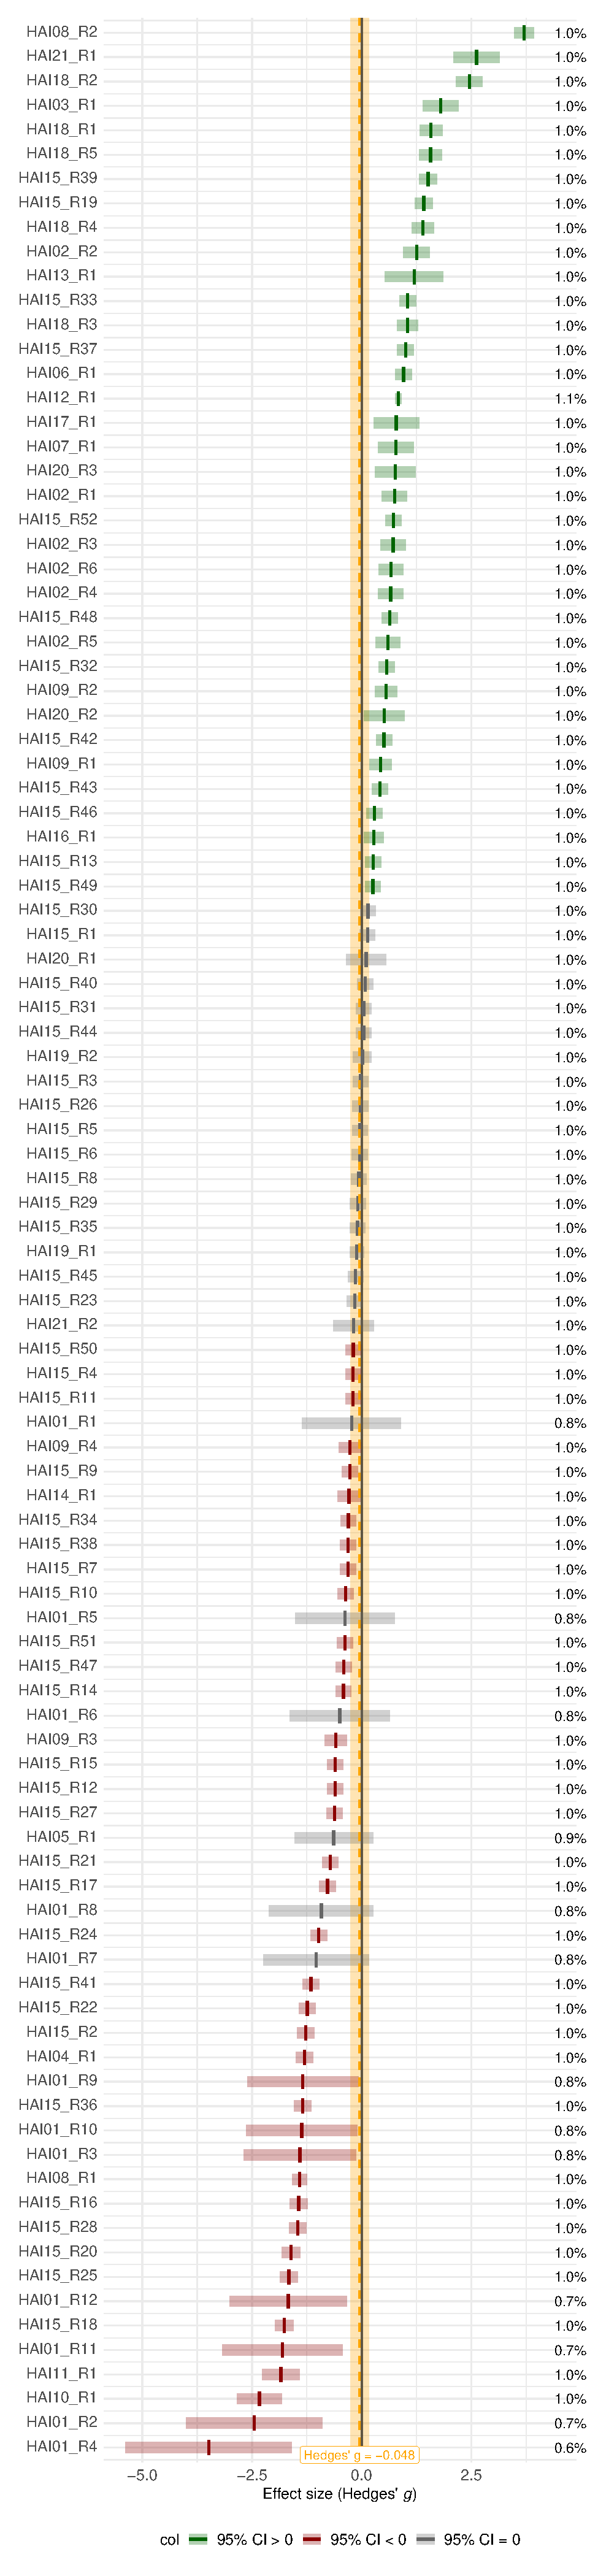
\includegraphics[width=\linewidth,
                 height=0.85\textheight,
                 keepaspectratio]{plot_versus_raw_forest}
  \caption{Forest plot summarising the Hedges' $g$ effect sizes and 95\% confidence intervals for direct Human vs. AI comparison at the replication level (Treatment: AI vs. Control: Human alone), across multiple individual replications of HAI tasks. Each line is one replication's estimate (weight at right), and the central diamond shows the overall effect size of $g$ = -0.050, indicating a negligible difference (slight disadvantage for AI). The vertical line at $g$ = 0 marks the null; points to the left favour the human control, to the right favour AI.}
  \label{fig:versus_raw_forest}
\end{figure}
\newpage
\subsubsection{Moderator Analysis}
\label{sec:CreativePerformanceComparisonOfHumanAndAI_Moderator}

\begin{figure}[h]
  \centering
  % (a) By GenAI model — includes Hedges' g axis label
  \begin{subfigure}[t]{0.33\linewidth}
    \centering
    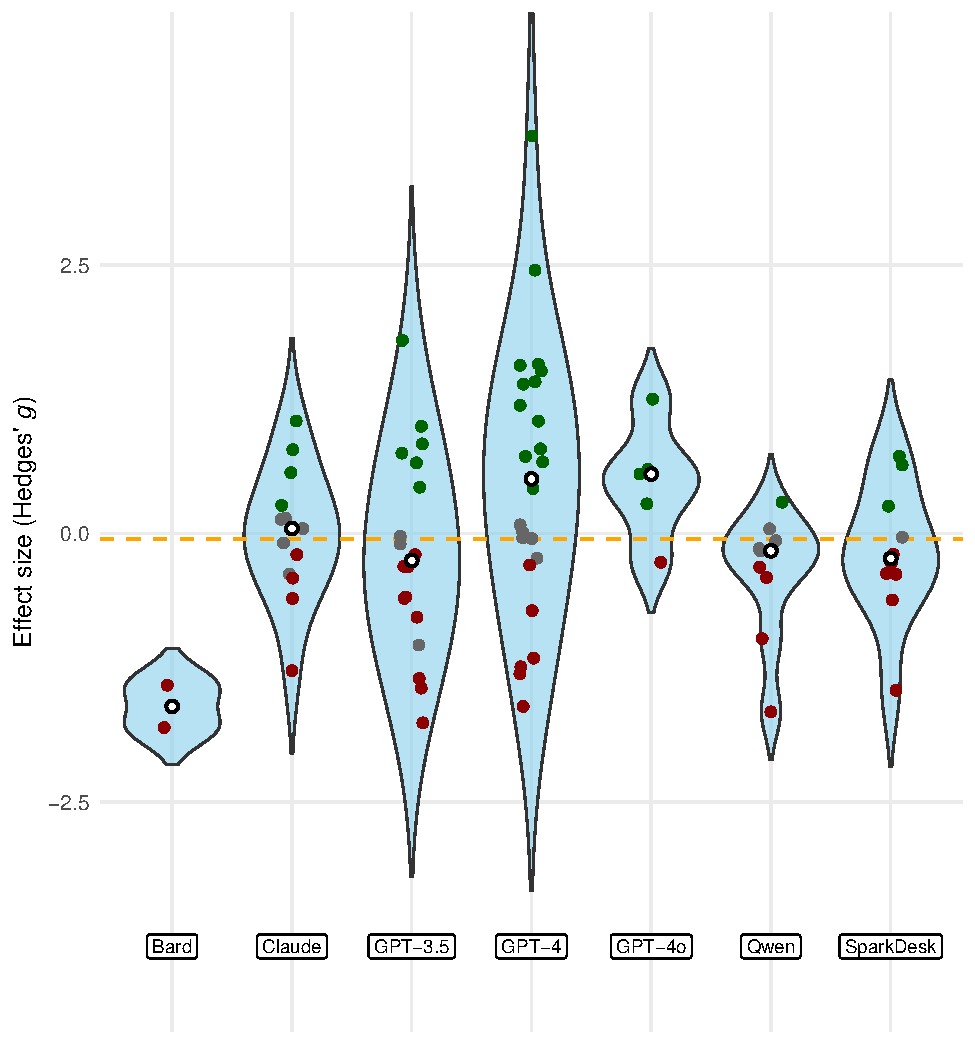
\includegraphics[width=\linewidth]{plot_versus_raw_violin_GenAI_Model}
    \caption{GenAI Model.}
    \label{fig:versus_violin_genai_model}
  \end{subfigure}\hfill
  % (b) By participant type
  \begin{subfigure}[t]{0.33\linewidth}
    \centering
    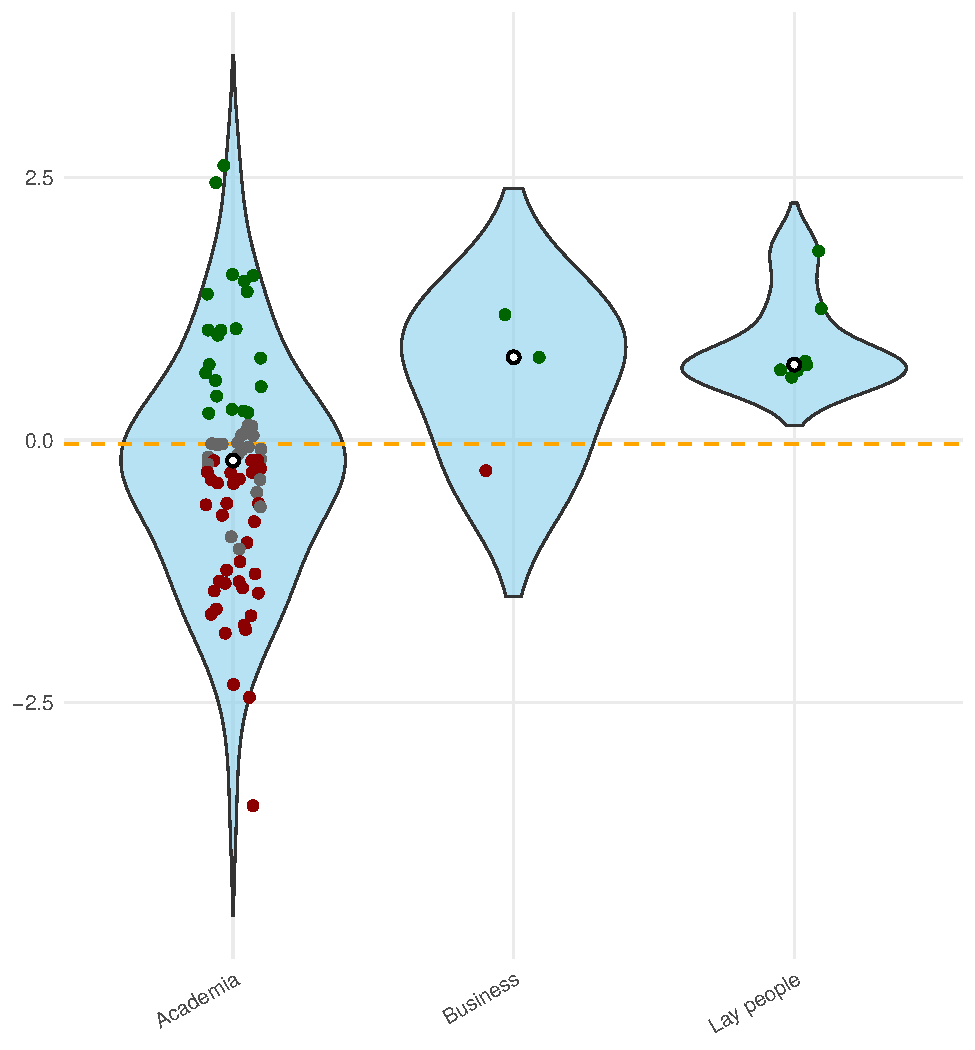
\includegraphics[width=\linewidth]{plot_versus_raw_violin_Participants}
    \caption{Participant Type.}
    \label{fig:versus_violin_participants}
  \end{subfigure}\hfill
  % (c) By creative task type
  \begin{subfigure}[t]{0.33\linewidth}
    \centering
    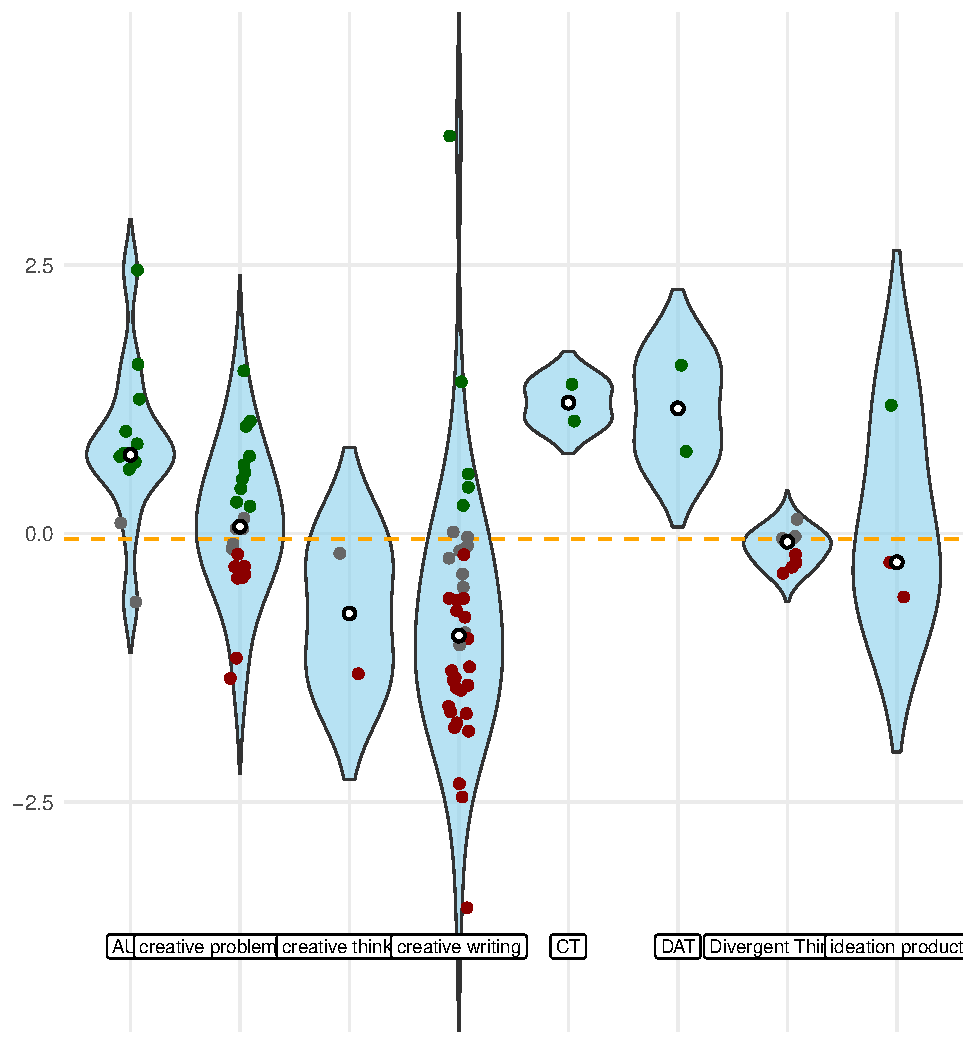
\includegraphics[width=\linewidth]{plot_versus_raw_violin_Task_Type}
    \caption{Task Type.}
    \label{fig:versus_violin_task_type}
  \end{subfigure}
  \caption{Violin plots showing the distribution of replication-level Hedges' \(g\) for direct Human vs.\ AI comparisons, stratified by (a) GenAI model, (b) participant type, and (c) creative task type. Widths reflect density of effect sizes; the dashed line at \(g=0\) marks no overall difference.}
  \label{fig:versus_raw_violins}
\end{figure}

\textbf{GenAI model:} As a expected key outcome influence we study the moderator of GenAI model. The model \textit{GPT‑4} performs the strongest with distribution centred slightly above zero. Meta-regression confirms the \textit{GPT‑4} distribution (\(g = 0.499,\;95\% [0.132, 0.865],\;p = 0.008\)). \textit{Bard} is measured to be the lowest performing GenAI model eligible for meta regression, with the coefficient (\(g = -1.570,\;95\% [-2.980, -0.151],\;p = 0.030\)), thereby being outperformed by humans. All other models overlap zero with wide tails and non‑significant coefficients, illustrating substantial within‑model variability. 

\textbf{Participants:} For the moderator participants \emph{lay people} appear to be constantly outperformed by GenAI (\(g = 0.918,\;95\% [0.202, 1.630],\;p = 0.012\)). Lay‑participant distribution is right‑skewed and centred above zero. While academics show a small but significant pro‑human difference (\(g = -0.223,\;95\% [-0.445, -0.001],\;p = 0.049\)), and business cohorts remain inconclusive (\(g = 0.539,\;95\% [-0.579, 1.660],\;p = 0.345\)) academic studies cluster modestly left of zero, and business samples span the full range, visually mirroring the mixed participant effects. Participant background thus moderates the AI–human gap in a non‑uniform manner. 

\textbf{Task type:} Violin shapes show modes above zero for AUT and CT tasks. The Alternate Uses Test favours AI (\(g = 0.855,\;95\% [0.358, 1.350],\;p < 0.001\)), as do CT tasks (\(g = 1.220,\;95\% [0.016, 2.420],\;p = 0.047\)). By contrast, creative‑writing tasks favour humans (\(g = -0.717,\;95\% [-1.010, -0.424],\;p < 0.001\)), a pronounced left‑shift for creative writing. Other categories (e.g., creative problem solving, divergent thinking) are non‑significant, highlighting task‑specific effects. The violin plot has a broad overlap for remaining categories, echoing the task‑specific moderator coefficients.

\subsubsection{Heterogeneity, Bias, and Robustness Diagnostics}
\textbf{Funnel plot \& Egger test:} Egger's mixed‑effects regression detects significant funnel asymmetry ($z=-3.363$, $p=0.001$), indicating the presence of small‑study or publication bias. The \textbf{Trim-and‑fill adjustment} therefore imputes 24 missing studies on the right of the funnel and shifts the random‑effects estimate to ($g=0.364$, 95 \% CI\,[\,$0.131$, $0.596$], $p=0.002$), implying that bias‑correction would reverse the direction of the overall effect in favour of AI. 
\textbf{Influence diagnostics:} All influence metrics (studentised residuals, DFFITS, Cook's $D$, hat values, cov.r) remain well below critical cut‑offs except for one flagged outlier; removing this study lowers $\tau^{2}$ only modestly (to $0.93$) and leaves the pooled effect virtually unchanged, confirming that no single study drives the results.

\subsection{RQ 2a : Creative Performance}
\label{sec:CreativePerformance}
For the \textbf{RQ 2a} How creative are ideas generated by humans when supported by GenAI (compared to humans without GenAI support)?  \\

\textbf{Forest plot.} The random‑effects meta‑analysis of $k=21$ human–AI collaboration studies yields a pooled Hedges\,$g = 0.273$ with 95 \% CI\,[0.018, 0.528] and $p = 0.036$; heterogeneity is substantial ($Q_{20}=232.17$, $p<0.001$, $I^{2}=94.11\,\%$, $\tau^{2}=0.3261$). No single study contributes more than 5.1 \% weight, indicating that the positive performance advantage is not driven by any single experiment. 

\textbf{Leave‑one‑out sensitivity.} Sequential deletion keeps the pooled effect between $g = 0.204$ and $g = 0.343$; in every iteration the 95 \% CI lower bound stays at or above 0.0004, and $I^{2}$ remains above 91 \%, confirming that the positive performance effect is stable yet accompanied by persistent heterogeneity.
\begin{figure}[H]
  \centering
  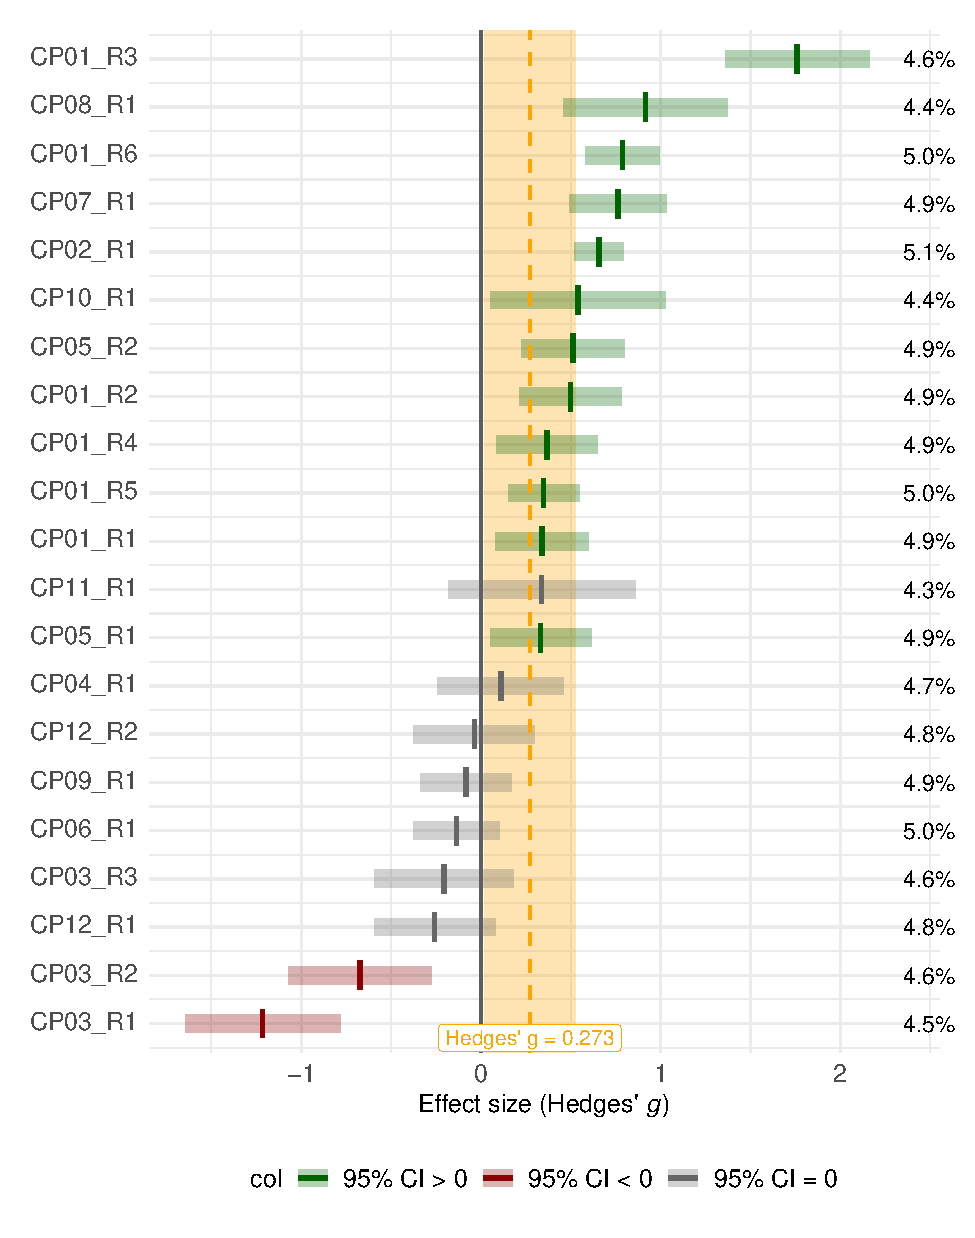
\includegraphics[width=\linewidth,
                 height=0.9\textheight,
                 keepaspectratio]{plot_performance_raw_forest}
  \caption{Forest plot summarising the Hedges' $g$ effect sizes and 95\% confidence intervals for creative performance at the replication level (Treatment: Human+AI vs Control: Human alone), across multiple replication trials for the fourteen tasks (e.g. CP01\_R1-CP14\_R4). Each line is one trial's estimate (weight at right), and the central diamond shows the overall effect size of $g$ = 0.219, indicating a modest performance gain from AI assistance. The vertical line at $g$ = 0 marks no effect; points to the right favour the AI-assisted treatment.}
  \label{fig:performance_raw_forest}
\end{figure}

\subsubsection{Moderator Analysis}
\begin{figure}[h]
  \centering
  % (a) Effect sizes by model — has the Hedges' g label
  \begin{subfigure}[t]{0.33\linewidth}
    \centering
    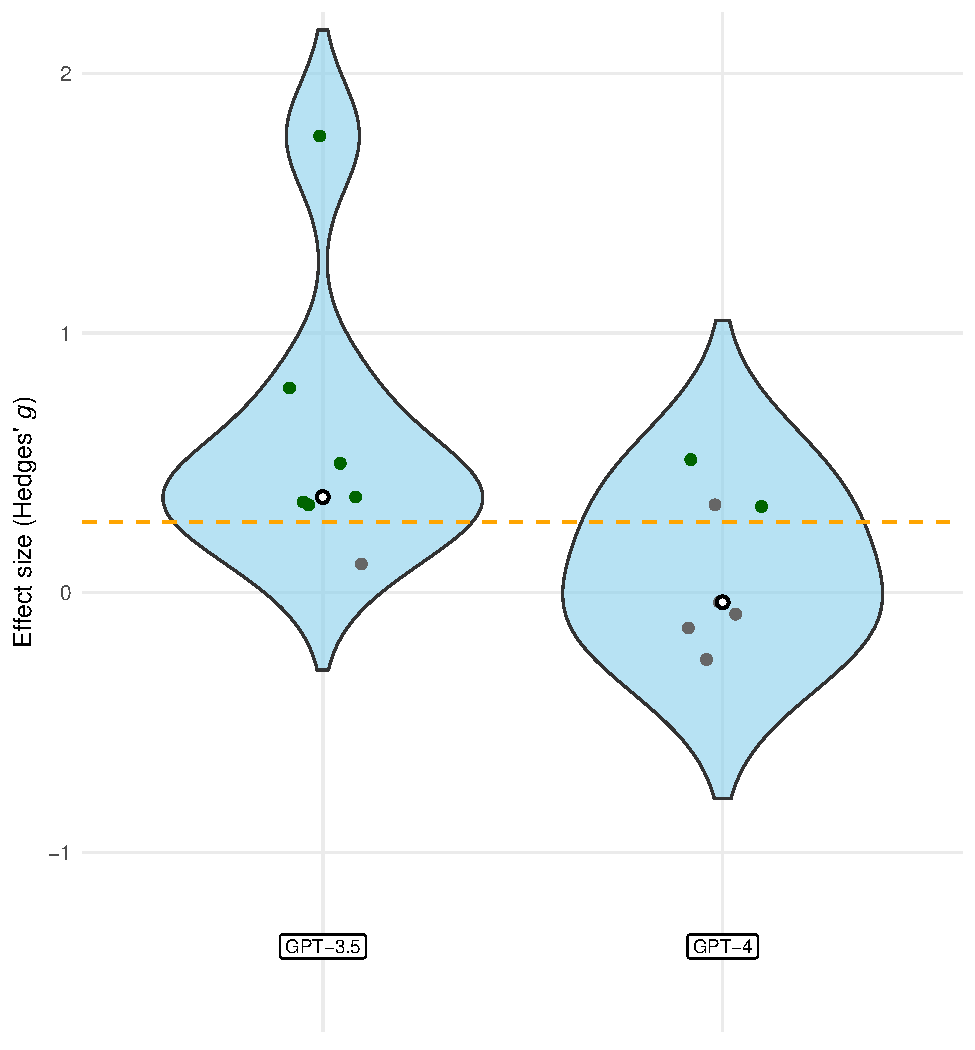
\includegraphics[width=\linewidth]{plot_performance_raw_violin_GenAI_Model}
    \caption{GenAI Model.}
    \label{fig:perf_violin_genai_model}
  \end{subfigure}\hfill
  % (b) By participant type
  \begin{subfigure}[t]{0.33\linewidth}
    \centering
    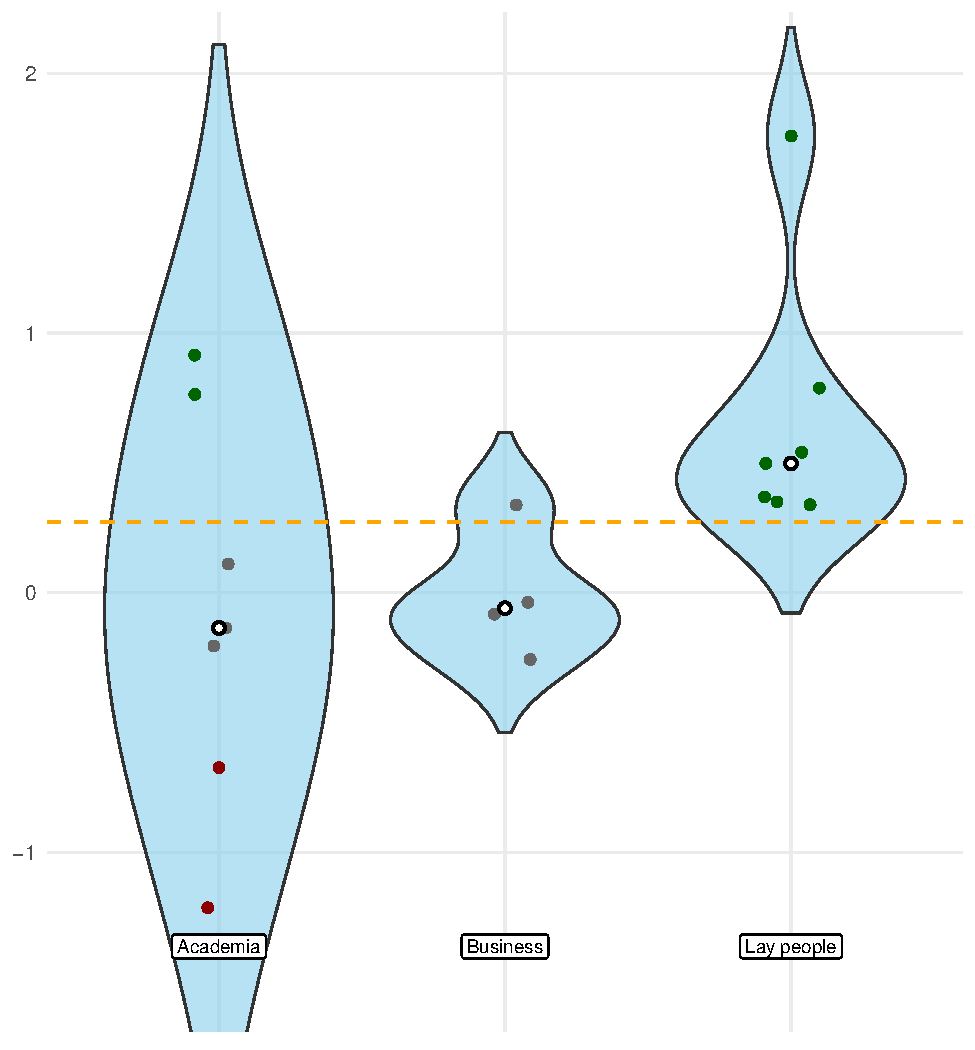
\includegraphics[width=\linewidth]{plot_performance_raw_violin_Participants}
    \caption{Partcipant Type.}
    \label{fig:perf_violin_participants}
  \end{subfigure}\hfill
  % (c) By creative task
  \begin{subfigure}[t]{0.33\linewidth}
    \centering
    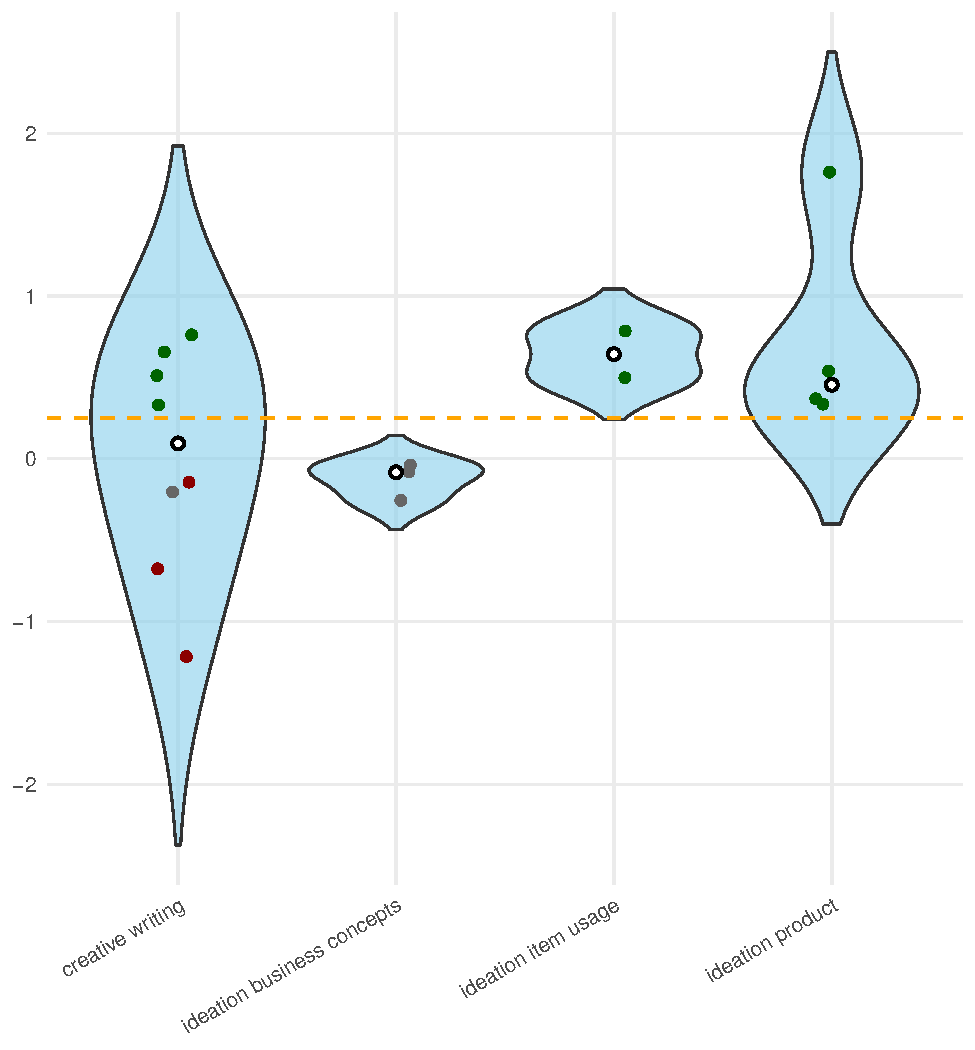
\includegraphics[width=\linewidth]{plot_performance_raw_violin_Task_Type}
    \caption{Task Type.}
    \label{fig:perf_violin_task_type}
  \end{subfigure}
  \caption{Violin plots of replication-level Hedges' \(g\) for direct Human vs.\ AI comparisons across different stratifications.  Widths reflect density of effect sizes; the dashed line at \(g=0\) marks no overall difference.}
  \label{fig:perf_raw_violins}
\end{figure}
\textbf{Violin plot—GenAI model.} Density ridges depict a higher median and thicker right tail for \textit{GPT‑3.5} relative to \textit{GPT‑4}, visually reinforcing the regression result that GPT‑3.5 contributes the strongest performance gains. 
\textbf{Moderator: GenAI model.} Deploying \textit{GPT‑3.5} significantly augments the performance benefit of human–AI teams (\(g = 0.587,\;95\% [0.280, 0.893],\;p < 0.001\)), whereas \textit{GPT‑4} shows no detectable deviation from the grand mean (\(g = 0.089,\;95\% [-0.223, 0.401],\;p = 0.577\)); thus only GPT‑3.5 explains a meaningful share of the between‑study variance.
\textbf{Violin plot—Participants.} Effect‑size distributions for \emph{lay people} are right‑skewed and centred above zero, while those for \emph{academia} and \emph{business} cluster tightly around the grand mean, mirroring the significant moderator effect for lay samples. 
\textbf{Moderator: Participants’ background.} Experiments with \emph{lay people} amplify the collaboration effect (\(g = 0.654,\;95\% [0.237, 1.070],\;p = 0.002\)), whereas studies recruiting from \emph{academia} (\(g = -0.057,\;95\% [-0.480, 0.367]\)) or \emph{business} settings (\(g = -0.021,\;95\% [-0.581, 0.540]\)) do not differ from baseline, indicating that participant expertise moderates outcomes asymmetrically. {index=3}
\textbf{Violin plot—Task type.} The widest and most right‑shifted violin corresponds to \emph{ideation—product} tasks, whereas \emph{creative writing} remains symmetric around zero; other ideation categories show broad overlap, visually corroborating task‑specific moderation patterns.
\textbf{Moderator: Task type.} Human–AI teams excel in \emph{ideation—product} tasks (\(g = 0.743,\;95\% [0.128, 1.360],\;p = 0.018\)), whereas \emph{creative writing} (\(g = 0.048,\;95\% [-0.412, 0.508]\)) and \emph{ideation—business concepts} tasks (\(g = -0.125,\;95\% [-0.826, 0.575]\)) show no significant moderation; \emph{ideation—item usage} trends positive but remains non‑significant.

\subsubsection{Heterogeneity, Bias, and Robustness Diagnostics}
\textbf{Funnel plot \& Egger test.} Egger’s regression detects no funnel asymmetry ($z=-0.624$, $p=0.533$), suggesting the absence of small‑study or publication bias. 

\textbf{Trim‑and‑fill analysis.} The procedure imputes zero missing studies; the bias‑adjusted estimate remains essentially unchanged at $g = 0.273$ with 95 \% CI\,[0.018, 0.528], corroborating the robustness of the performance benefit.

\textbf{Influence diagnostics.} One observation shows a high studentised residual ($r = 2.933$), but its removal reduces $\tau^{2}$ only from 0.3261 to 0.2271 and leaves $g$ within the original confidence limits; all other influence metrics (DFFITS, Cook’s $D$, hat values, cov.r) remain below conventional thresholds. 

\subsection{RQ 2b :Creative Diversity}
\label{sec:CreativeDiversity}

\textbf{RQ 2b:} How does using GenAI affect idea diversity in creativity tasks? \\
\textbf{Strong limitation due to small amount of studies available}

\textbf{Forest plot.} The six human–AI collaboration studies yield a pooled Hedges\,$g = -0.863$ with 95 \% CI\,[\,-1.328, -0.398] and $p < 0.001$; heterogeneity is severe ($Q_{5}=51.69$, $p<0.001$, $I^{2}=93.70\,\%$, $\tau^{2}=0.310$). Each study carries roughly 16–17 \% weight, confirming a consistent and statistically meaningful reduction in idea diversity when AI joins the team. 

\textbf{Influence diagnostics.} One outlier (study \#4) shows a studentised residual of $-3.662$ and Cook’s $D = 0.766$; excising it lowers $\tau^{2}$ from 0.310 to 0.067 and $Q_{E}$ from 51.69 to 17.87, but the pooled effect remains negative and significant ($g = -0.656$, 95 \% CI\,[\,-0.913, -0.398]). Thus, although the outlier inflates heterogeneity, it does not alter the substantive conclusion. 

\textbf{Leave‑one‑out sensitivity.} Sequential deletion keeps the pooled estimate between $g = -0.655$ and $g = -0.952$; every 95 \% CI excludes zero, and $I^{2}$ never falls below 78.21 \%. The diversity‑reducing effect is therefore robust to removal of any single study, albeit heterogeneity persists. 


\begin{figure}[H]
  \centering
  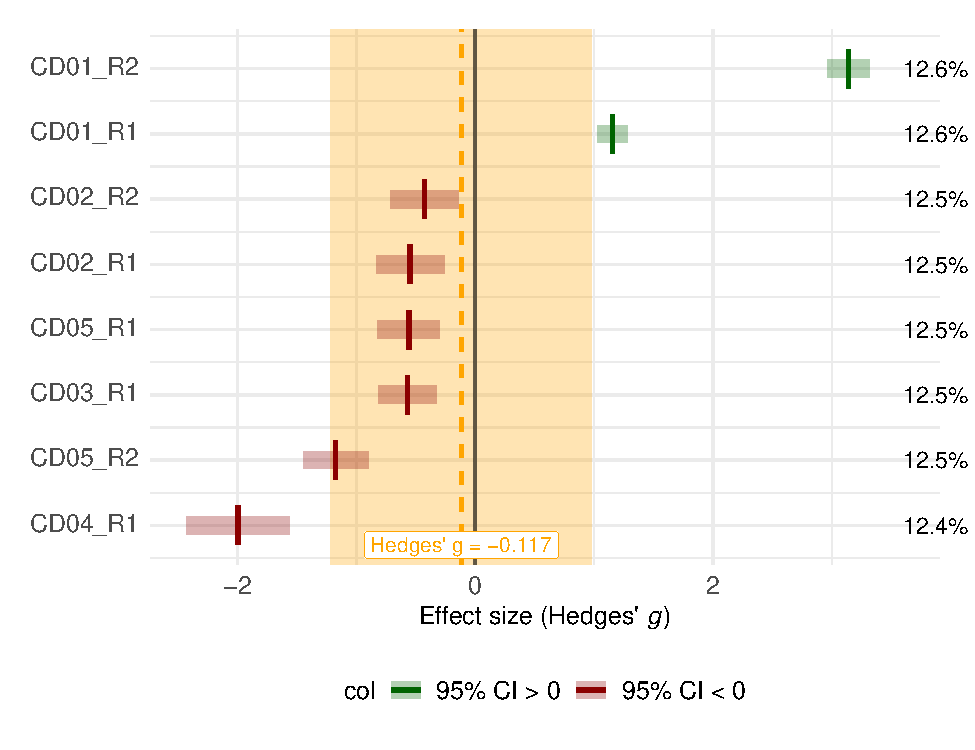
\includegraphics[width=\linewidth]{plot_diversity_raw_forest}
  \caption{Forest plot summarising the Hedges' $g$ effect sizes and 95\% confidence intervals for creative diversity at the replication level (Treatment: Human+AI vs. Control: Human alone), across five individual replications (CD01\_R1, CD02\_R1, CD02\_R2, CD03\_R1, CD04\_R1). Each line is one replication's estimate (weight at right), and the central diamond is the overall effect size of $g$ = 2.139, indicating a substantial diversity gain from AI assistance. The vertical line at $g$ = 0 marks the null—rightwards points favour the AI-assisted treatment.}
  \label{fig:diversity_raw_forest}
\end{figure}

\subsubsection{Moderator Analysis}
\label{sec:CreativeDiversity_Moderator_GenAI}

\textbf{Moderator: Participants.} Compared with lay samples, academic cohorts show a markedly stronger reduction in diversity (\(g = -1.260,\;95\% [-2.340, -0.187],\;p = 0.021\)), while business populations exhibit a non‑significant shift (\(g = -0.866,\;95\% [-1.930, 0.197],\;p = 0.110\)); participant background thus moderates the magnitude of the negative diversity effect. 

\newpage

\subsection{Overall Results}


\begin{table}[H]
  \centering
  % latex table generated in R 4.2.3 by xtable 1.8-4 package
% Sun May 11 17:11:47 2025
\begin{table}[H]
\centering
\begin{tabular}{lrrrrrrrrr}
  \toprule
Analysis & Effect & SE & ci95 & p (sig) & Q & df & pQ & i2 & tau2 \\ 
  \midrule
Performance & 0.18 & 0.09 & [-0.003,0.363] & 0.054 & 377.59 & 30.00 & 0.00 & 93.70 & 0.25 \\ 
  Diversity & 0.71 & 0.14 & [0.442,0.977] & 0.000*** & 39.96 & 4.00 & 0.00 & 85.40 & 0.08 \\ 
  Human\_vs\_AI & -0.05 & 0.12 & [-0.285,0.186] & 0.679 & 7102.56 & 94.00 & 0.00 & 99.10 & 1.31 \\ 
   \bottomrule
\end{tabular}
\caption{Raw‐level meta‐analysis results for each outcome. Hedges’ $g$, standard errors, 95\% CIs, p‐values, and heterogeneity statistics (Q, df, pQ, I\textsuperscript{2}, $\tau^2$).} 
\label{tab:meta_raw}
\end{table}

\end{table}

\section{Discussion}
\label{sec:discussion}

\subsection{Summary of Key Findings}

The fragmented state of the literature in human-AI co-creativity research raises two central questions: \textit{How creative are the ideas generated by GenAI? And to what extent can GenAI support humans in producing ideas that are both creative and diverse?} For our meta-analysis, we screened 693 records and finally included \TODO{Niklas} studies (with \TODO{NIKLAS: $N=$ subjects}) comparing creative performance along three dimensions: (i)~how creative GenAI is, (ii)~how creative human+GenAI collaboration is vs. human-only performance, and (iii)~the effect of human+GenAI collaboration on idea diversity.

\begin{table}[H]
\centering
\footnotesize
\begin{tabular}{@{}llcc@{}}
  \toprule
RQ  & Description                        & Hedges' $g$       & Supported? \\ 
  \midrule
RQ1 & Creative performance of GenAI (compared to human)            & $-0.04$ (ns)      & \textcolor{BrickRed}{\ding{55}} \\ 
RQ2a & Creative performance of human+GenAI (compared to human only)            & $0.25^{*}$      & \textcolor{ForestGreen}{\ding{51}} \\ 
RQ2b & Diversity of ideas in human+GenAI (compared to human only)              & $-0.86^{***}$      & \textcolor{ForestGreen}{\ding{51}} \\ 
  \bottomrule
\end{tabular}
\caption{\textbf{Key findings from our meta-analysis.} Reported are Hedges' $g$ for each anaysis. \textcolor{ForestGreen}{\ding{51}} indicates $p< 0.001$, \textcolor{BrickRed}{\ding{55}} indicates non-significant. Significance levels: $^{***}$: $p < 0.001$; $^{**}$: $p < 0.01$; $^{*}$: $p < 0.05$.}
\label{tab:rq_overview}
\end{table}


\textbf{Finding for RQ1: Parity rather than super-human creativity.} GenAI matches the average human creative output ($g \approx 0$; see Table~\TODO{NIKLAS}). A moderate advantage ($g \approx $\TODO{NIKLAS: Wert aus dem deepdive}) emerges only for specific GenAI models and is largely attributable to a subset of studies using GPT-4o. Hence, any observed superiority is tied to specific models, rather than being a general property of LLMs. This result is also in line with studies explicitly comparing the creative performance of different models, like ChatGPT-3 and ChatGPT-4 \cite{Koivisto.2023}. Nevertheless, with the growing number of research using recent LLMs with reasoning capabilities, we may observe a gradual shift in average performance benchmarks. 

\textbf{Finding to RQ2a. Modest but robust gains from collaboration.} Human-AI teams deliver a small yet robust boost in creative performance ($g\approx 0.17$) that holds across different models, tasks, and participant backgrounds. While our meta-analysis focused on comparing human-AI collaboration with human-only performance (rather than contrasting human-AI teams with AI-only outputs), recent studies examining the latter report no significant performance gains from adding humans to AI-generated content  \cite{LeeChung2024}. Together, humans using AI therefore show higher creative performance than humans without AI support.

\textbf{Finding to RQ2b. Decrease in idea diversity.} Our meta-analysis finds no statistically significant effect of GenAI on idea diversity \TODO{nicht consistent mit tabelle -- bitter checken}($g = -0.12$). While four studies indicate a potential homogenization effect of GenAI use on idea diversity, one study does not. However, given the small number of available studies, it remains unclear whether the observed trend reflects specific study configurations (e.g., GPT-4 use together wtih text-based tasks) or whether it indicates a more generalizable pattern. As such, our findings are consistent with prior work on GenAI-powered writing assistants \TODO{e.g. cite https://doi.org/10.1145/3544548.3581196}, where GenAI exerts a strong influence on human behavior and \TODO{???? which may limit diversity in the produced texts}. 



\subsection{Implications}

\textbf{Practical implications:} Our research suggests substantial potential for organizations to integrate GenAI into creative workflows---but only by pairing it with employees to enhance ideation processes. These benefits also imply a shift in individual creative potential: as AI can augment human creativity, especially lower innate creative capabilities might be compensated \TODO{included citation on study that analyzed different skills}. Yet, the observed gains in creativity could come at a cost, namely, in the form of a reduction in idea diversity. As a result, users collaborating with GenAI tend to produce more homogeneous outputs in some settings. This trade-off is especially problematic in contexts where ideational breadth is essential, such as where companies search for ``out-of-the-box'' ideas such as in open innovation and crowd ideation tasks \TODO{include citation, http://europepmc.org/abstract/MED/23593768}. Thus, while AI-human teaming may suffice for boosting individual creativity, practitioners will need to be careful when scaling GenAI use with the intention of promoting collective creativity.

Further, current GenAI models often tend to recombine familiar elements \cite{LeeChung2024} across contexts rather than generating radically novel ideas, which may lead to more incremental innovation. This highlights the importance of human agency in co-creation processes to counteract potential convergence effects---where repeated exposure to similar outputs leads to reduced variability---and highlights the need for human-AI systems that actively support diversity.


\textbf{Theoretical implications:} Our study reveals that the creative impact of GenAI is highly contingent on contextual factors. A high between-study heterogeneity $I^{2}$ >80 \% demonstrates that creativity augmentation cannot be treated as a general affordance of GenAI alone. However, the effectiveness mechanisms of GenAI in creativity remain unclear. Importantly, our heterogeneity analysis identifies only the choice of the GenAI model as a consistent moderator that explains higher creativity levels. 

Given that the benefit from human-AI collaboration in creative tasks is robust for both laypeople and domain experts, it is likely that the performance gain is due to a generic facilitation mechanism (e.g. faster drafting and broader ideation, reduced cognitive load) rather than task-specific benefits from augmentation. Previous evidence indicates that co-creation tasks are particularly beneficial for human-AI collaboration when there are inherent synergies between humans and AI systems, allowing each to leverage their respective strengths---unlike in many analytical, decision-making contexts  \TODO{(cite: https://www.nature.com/articles/s41562-024-02024-1)}.

%These findings shift the theoretical focus from general capabilities of GenAI to the conditions under which it becomes a productive collaborator. 

\subsection{Limitations and Future Research}

Our meta-analysis has limitations due to the current state of research and technological progress. First, some of the included studies are not yet peer-reviewed. Nevertheless, we still chose to include them to provide a timely synthesis of empirical findings including recent ones. Second, the findings depend on the choice of GenAI models. Given the fast-evolving capabilities of GenAI, it is likely that newer models, including different reasoning capabilities or different fine-tuning strategies, may yield different outcomes. Third, many studies use simple, well-known tasks for benchmarking such as the so-called alternative uses test, which asks participants to generate creative uses for common objects. Such tasks may have been part of the training data in GenAI models, which is a known issue in GenAI research \TODO{cite: https://arxiv.org/abs/2406.04244} and underscores the need for devising novel tasks that preserve experimental rigor while minimizing overlap with model training data.


To guide future work, we identified salient gaps around the use of AI for creativity systems in HCI/CSCW research based on our structured literature review and propose three key research directions.

\textbf{Research direction 1: \textit{More relevant, real-world-inspired study designs:}} The majority of studies focus on simplified creativity tasks such as the alternative uses test (AUT) \TODO{(e.g., as used in [example paper])} and divergent thinking exercises \TODO{(e.g., as used in [example paper])}. While these tasks draw on established scales from psychological research to assess creativity, they fall short of capturing the complexity of real-world settings that involve creative thinking. In contrast, there are only a few studies that test GenAI in real-world situations such as work settings (the only exception is \TODO{xyz}, where the task was yz), or with creative tasks beyond text, such as images, audio, or code (with the exception of REF). 

Future studies could focus on more realistic scenarios for a higher ecological validity and further explore context-sensitive moderators for more targeted creativity interventions. For example, to enhance relevance to CSCW and HCI applications in business contexts, future studies could investigate settings where tacit knowledge plays a critical role, or where creative tasks must account for specific organizational contexts---such as operational constraints or strategic alignment. One promising direction would be to examine how GenAI can support ideation in tasks like developing new business models that align with a company's brand strategy or existing capabilities of that company. Moreover, all of the existing studies were performed at a single time point; thus, longitudinal designs are needed to examine how collaboration patterns and creativity effects evolve over time---especially as users gain fluency in leveraging GenAI within creative tasks.

 
    
\textbf{Research direction 2: \textit{Understand psychological mechanisms:}} Existing research has primarily focused on the outcomes of GenAI-assisted creativity, typically through rigorous A/B experiments. Yet, prior research has largely overlooked the underlying psychological mechanisms that drive the effects. For example, it is unclear whether gains in GenAI-assisted creativity come from broader ideation (e.g., generating more ideas due to increased speed or reduced distractions), deeper engagement (e.g., more intensive thinking due to reduced cognitive load), or heightened motivation (e.g., playful interaction with the system). 

To develop a more nuanced understanding of human-AI co-creation, future work should explore potential psychological mediators and moderators, such as cognitive effort, user agency, trust, task framing, and participant's personality traits. Uncovering such cognitive processes is relevant to identifying how human and machine capabilities can be combined to foster synergistic collaboration. Ultimately, such insights could inform frameworks with a notion of `appropriate reliance' (see \TODO{cite: https://dl.acm.org/doi/10.1145/3581641.3584066} for an overview on the notion of appropriate reliance in AI advance), that is, when it is most beneficial for an idea to originate from the human, the AI system, or through their interaction.
    
\textbf{Research direction 3: \textit{Explore CSCW/HCI design choices to elicit creative thinking:}} The majority of studies identified in our literature review rely on relatively naive GenAI setups---often based on simple one-shot prompts (e.g., as in \TODO{example paper}) or by providing participants with unmodified, off-the-shelf LLMs (e.g., as in \TODO{example}). In contrast, studies that devise and compare different design choices are largely absent. Future studies could thus explore more elaborate workflows (e.g., critique-refine, suggestions-refine) that reflect an iterative creation process. Eventually, this could help to integrate GenAI tools into creativity systems through effective, user-friendly interfaces that allow for natural interactions, as well as to build AI agents that are effective at supporting creative thinking tasks.



\section{Conclusion}
\label{sec:conclusion}

Our meta-analysis shows that GenAI and humans show similar creative performance on average, with moderate advantages emerging mainly for GPT-4. In contrast, human-AI collaboration shows small but consistent gains in creative output across tasks and contexts. However, collaboration with GenAI reduces the diversity of ideas, indicating a risk of creative outputs that could become more homogeneous. Our meta-analysis also highlights important gaps in the literature, which provide interesting avenues for future research to the understand psychological mechanisms of human-AI augmentation and identify drivers for how GenAI system can successfully elicit creative thinking.

\newpage
\bibliographystyle{ACM-Reference-Format}
\bibliography{metaanalysis_llm_creativity}

\newpage
\TODO{Acknowledgment of AI usage for Paper}\\
\TODO{Acknowledgment Review was not registered (thereby no changes made) - No Review Protocol}\\
\TODO{Acknowledgment No funding - Support Prof. Feuerriegel}\\
\TODO{Acknowledgment No competing intrests}\\
\TODO{GitHub Data-avaliability}
\appendix
\section{Descriptive statistics Moderators}
\subsection{GenAI Type}
\begin{table}[H]
  \centering
  % latex table generated in R 4.2.3 by xtable 1.8-4 package
% Tue May 20 13:57:18 2025
\begin{table}[ht]
\centering
\label{tab:GenAI_Type}
\begin{tabular}{lrrrr}
  \toprule
Characteristic & Creative_Performance & Creative_Diversity & Human_vs_AI & Total \\ 
  \midrule
T2T &  21 &   6 & 100 & 127 \\ 
   \bottomrule
\end{tabular}
\end{table}

\end{table}
\subsection{GenAI Model}
\begin{table}[H]
  \centering
  % latex table generated in R 4.2.3 by xtable 1.8-4 package
% Wed May 14 08:33:23 2025
\begin{table}[ht]
\centering
\label{tab:GenAI_Model}
\begin{tabular}{lrrrr}
  \toprule
Characteristic & Creative_Performance & Creative_Diversity & Human_vs_AI & Total \\ 
  \midrule
GPT-4 &   7 &   5 &  25 &  37 \\ 
  GPT-3.5 &   7 &   0 &  18 &  25 \\ 
  Claude &   0 &   0 &  13 &  13 \\ 
  SparkDesk &   0 &   0 &  10 &  10 \\ 
  Qwen &   0 &   0 &   9 &   9 \\ 
  > 5 models &   0 &   1 &   6 &   7 \\ 
  GPT-4o &   0 &   0 &   5 &   5 \\ 
  n.d. &   3 &   0 &   1 &   4 \\ 
  2 Models &   2 &   0 &   0 &   2 \\ 
  Bard &   0 &   0 &   2 &   2 \\ 
  3 models &   0 &   0 &   1 &   1 \\ 
  5 models &   0 &   0 &   1 &   1 \\ 
  Dou Bao &   1 &   0 &   0 &   1 \\ 
  GPT-3 &   0 &   0 &   1 &   1 \\ 
  GPT-3.5-turbo &   1 &   0 &   0 &   1 \\ 
  GPT-4all &   0 &   0 &   1 &   1 \\ 
  alpaca &   0 &   0 &   1 &   1 \\ 
  bing &   0 &   0 &   1 &   1 \\ 
  dolly &   0 &   0 &   1 &   1 \\ 
  koala &   0 &   0 &   1 &   1 \\ 
  oa &   0 &   0 &   1 &   1 \\ 
  stablelm &   0 &   0 &   1 &   1 \\ 
  vicuna &   0 &   0 &   1 &   1 \\ 
   \bottomrule
\end{tabular}
\end{table}

\end{table}
\subsection{Measurement Evaluators}
\begin{table}[H]
  \centering
  % latex table generated in R 4.2.3 by xtable 1.8-4 package
% Tue May 13 16:15:42 2025
\begin{table}[ht]
\centering
\label{tab:Measurement_Evaluator}
\begin{tabular}{lrrrr}
  \toprule
Characteristic & Creative_Performance & Creative_Diversity & Human_vs_AI & Total \\ 
  \midrule
Human &   7 &   0 &  73 &  80 \\ 
  Expert &  13 &   0 &  17 &  30 \\ 
  Rule-based &   1 &   8 &   6 &  15 \\ 
  AI &   0 &   0 &   5 &   5 \\ 
  Self-assessed &   1 &   0 &   0 &   1 \\ 
   \bottomrule
\end{tabular}
\end{table}

\end{table}
\subsection{Creativity Measurement}
\begin{table}[H]
  \centering
  % latex table generated in R 4.2.3 by xtable 1.8-4 package
% Tue May 13 16:15:42 2025
\begin{table}[ht]
\centering
\label{tab:Creativity_Measurement}
\begin{tabular}{lrrrr}
  \toprule
Characteristic & Creative_Performance & Creative_Diversity & Human_vs_AI & Total \\ 
  \midrule
originality scale &   0 &   0 &  45 &  45 \\ 
  creativity scale &  13 &   0 &  30 &  43 \\ 
  novelty scale &   7 &   0 &  18 &  25 \\ 
  sematic distance &   0 &   0 &   8 &   8 \\ 
  cosine similarity &   0 &   6 &   0 &   6 \\ 
  cosine distance &   0 &   2 &   0 &   2 \\ 
  CPS scale &   1 &   0 &   0 &   1 \\ 
  felxibility score &   1 &   0 &   0 &   1 \\ 
   \bottomrule
\end{tabular}
\end{table}

\end{table}
\subsection{Task Type}
\begin{table}[H]
  \centering
  % latex table generated in R 4.2.3 by xtable 1.8-4 package
% Tue May 13 16:15:42 2025
\begin{table}[ht]
\centering
\label{tab:Task_Type}
\begin{tabular}{lrrrr}
  \toprule
Characteristic & Creative_Performance & Creative_Diversity & Human_vs_AI & Total \\ 
  \midrule
creative writing &   8 &   5 &  39 &  52 \\ 
  creative problem solving &   1 &   0 &  24 &  25 \\ 
  AUT &   0 &   0 &  12 &  12 \\ 
  ideation other &   3 &   2 &   6 &  11 \\ 
  Divergent Thinking &   0 &   0 &  10 &  10 \\ 
  ideation product &   4 &   0 &   3 &   7 \\ 
  ideation business concepts &   3 &   0 &   0 &   3 \\ 
  CT &   0 &   0 &   2 &   2 \\ 
  DAT &   0 &   0 &   2 &   2 \\ 
  creative thinking &   0 &   0 &   2 &   2 \\ 
  ideation item usage &   2 &   0 &   0 &   2 \\ 
  ideation research proposal &   1 &   1 &   0 &   2 \\ 
  FF &   0 &   0 &   1 &   1 \\ 
   \bottomrule
\end{tabular}
\end{table}

\end{table}
\subsection{Recruitment Source}
\begin{table}[H]
  \centering
  % latex table generated in R 4.2.3 by xtable 1.8-4 package
% Fri May 16 02:30:55 2025
\begin{table}[ht]
\centering
\label{tab:Recruitment_Source}
\begin{tabular}{lrrrr}
  \toprule
Characteristic & Creative_Performance & Creative_Diversity & Human_vs_AI & Total \\ 
  \midrule
University &   3 &   1 &  66 &  70 \\ 
  Prolific &  12 &   5 &  25 &  42 \\ 
  Public &   2 &   0 &   8 &  10 \\ 
  Mturk &   3 &   0 &   0 &   3 \\ 
  Company &   1 &   0 &   1 &   2 \\ 
   \bottomrule
\end{tabular}
\end{table}

\end{table}
\subsection{Participants}
\begin{table}[H]
  \centering
  % latex table generated in R 4.2.3 by xtable 1.8-4 package
% Fri May 16 02:28:13 2025
\begin{table}[ht]
\centering
\label{tab:Participants}
\begin{tabular}{lrrrr}
  \toprule
Characteristic & Creative_Performance & Creative_Diversity & Human_vs_AI & Total \\ 
  \midrule
Academia &   7 &   2 &  76 &  85 \\ 
  Not disclosed &   3 &   2 &  14 &  19 \\ 
  Lay people &   7 &   0 &   7 &  14 \\ 
  Business &   4 &   2 &   3 &   9 \\ 
   \bottomrule
\end{tabular}
\end{table}

\end{table}
\end{document}